\chapter{Compiled and Interpreted Languages}
\label{chap:compiled-interpreted}

A computer can directly execute only machine code, consisting of raw
numeric data.  Machine code can be written by humans, but we usually
use symbolic \textit{assembly languages} to make it more approachable.
However, even when using an assembly language, this form of
programming is very tedious.  This is because assembly languages are
(almost) a transparent layer of syntax on top of the raw machine code,
and the machine code has been designed to be efficient to
\textit{execute}, not to be a pleasant programming experience.
Specifically, we are programming at a very low level of abstraction
when we use assembly languages, and with no good ability to build new
abstractions.  In practice, almost all progamming is conducted in
\textit{high-level languages}.

\section{Low-level and High-Level Languages}

For the purpose of this chapter, a high-level programming language is
a language that is designed not to directly represent the capabilities
and details of some machine, but rather to \textit{abstract} the
mechanical details, in order to make programming simpler.  However, we
should note that ``high-level'' is a spectrum.  In general, the
meaning of the term ``high-level programming language'' depends on the
speaker and the context (\cref{fig:koronkebitch}).  The pioneering
computer scientist Alan Perlis said: \textit{``A programming language
  is low-level when its programs require attention to the
  irrelevant''}.  During the course you will gain familiarity with the
programming language C, which \textit{definitely} requires you to pay
attention to things that are often considered irrelevant, which makes
it low-level in Perlis's eyes.  However, we will see that the control
offered by C provides some capabilities, mostly the ability to
\textit{tune} our code for high performance, that are for some
problems \textit{not} irrelevant.  The term \textit{mid-level
  programming language} might be a good description of C, as it fills
a niche between low-level assembly languages, and high-level languages
such as Python and F\#.

\begin{figure}
  \centering
  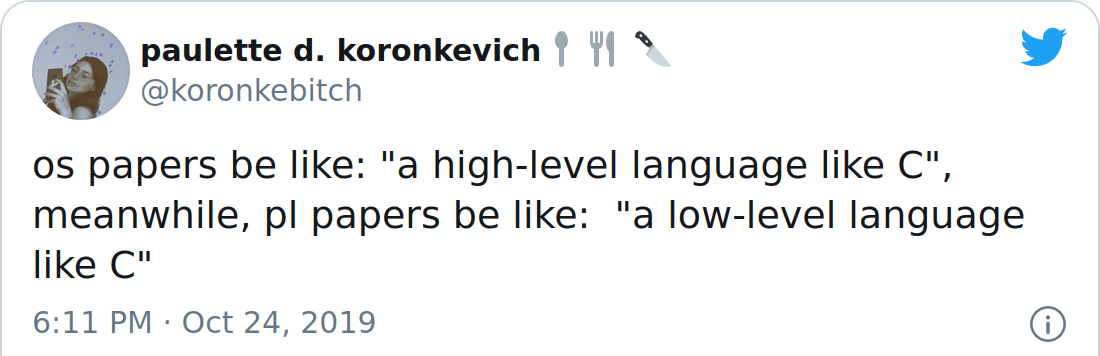
\includegraphics[width=\textwidth]{img/highleveltweet.png}
  \caption{A remark on the clarity of terms in computer science.}
  \label{fig:koronkebitch}
\end{figure}

Generally speaking, low-level languages tend to be more
\textit{difficult} to program in, while offering greater potential
\textit{performance} (i.e. programs written in them are faster).
Higher-level languages are much easier to program in, but run slower
and require more machine resources (e.g. memory).  Given the speed of
modern computers, this is a price we are often willing to
pay---especially in the common case where the slowest part of our
program is waiting for information from disk or network.  Do not make
the mistake of assuming that a program written in a low-level language
is \textit{always} faster than one written in a high-level language.
Choice of algorithm is often more important than choice of language.
Further, some high-level languages are specifically designed to
execute very efficiently.  But there is no free lunch: these languages
make tradeoffs in other areas.  There is no objective measure of where
a language lies on the scale of ``level-ness'', so while a statement
such as \textit{``Python is more high-level than C''} is unlikely to
raise any objections, it is usually pointless to try to rank very
similar languages on this spectrum.

\section{Compilers and Interpreters}

As the computer natively understands only its machine code, other
languages must be \textit{translated} to machine code in order to run.
For historical reasons, this is called \textit{compilation}.  We say
that a compiler takes as input a file with a \textit{source program},
and produces a file containing an executable \textit{machine program}
that can be run directly.  This is a very simplified model, for the
following reasons:

\begin{enumerate}
\item Strictly speaking, a compiler does not have to produce machine
  code.  A compiler can also produce code in a different high level
  languag.  For example, with the rise of browsers, it has become
  common to write compilers that produce JavaScript code.
\item The machine program normally cannot be \textit{directly}
  executed, as modern systems have many layers of abstraction on top
  of the processor.  While the compiler does produce machine code, it
  is usually stored in a special file format that is understood by the
  \textit{operating system}, which is responsible for making the
  machine code available to the processor.
\item The actual compiler contains many internal steps.  Further,
  large programs are typically not compiled all at once, but rather in
  chunks.  Typically, each \textit{source file} is compiled to one
  \textit{object file}, which are finally \textit{linked} to form an
  executable program.
\end{enumerate}

While compilers are a fascinating subject in their own right, we will
discuss them only at a superficial level.  For a more in-depth
treatment, you are encouraged to read a book such as Torben Mogensen's
\textit{Basics of Compiler
  Design}\footnote{\url{http://hjemmesider.diku.dk/~torbenm/Basics/}}.

In contrast, an \textit{interpreter} is a program that executes code
directly, without first translating it.  The interpreter can be a
compiled program, or itself be interpreted.  At the bottom level, we
always have a CPU executing machine code, but there is no fundamental
limit to how many layers of interpreters we can build on top.
However, the most common case is that the interpreter is a machine
code program, typically produced by a compiler.  For example, Python
is an interpreted language, and the \texttt{python} interpreter
program used by most people is written in C, and compiled to machine
code.

Interpreters are generally easier to construct than compilers,
especially for very dynamic languages such as Python.  The downside is
that code that is interpreted generally runs much slower than machine
code.  This is called the \textit{interpretive overhead}.  When a C
compiler encounters an integer expression \texttt{x + y}, then this
can likely be translated to a single machine code
instruction---possibly preceded by instructions to read \texttt{x} and
\texttt{y} from memory.  In contrast, whenever the Python interpreter
encounters this expression, it has to analyse it and figure out what
is supposed to happen (integer addition), and then dispatch to an
implementation of that operation.  This is usually at least an order
of magnitude slower than actually doing the work.  This means that
interpreted languages are usually slower than compiled languages.
However, many programs spend most of their time waiting for user
input, for a network request, or for data from the file system.  Such
programs are not greatly affected by interpretive overhead.

As an example of interpretive overhead, let us try writing programs
for investigating the Collatz conjecture.  The Collatz conjecture
states that if we repeatedly apply the function
\[
  f(n) =
  \begin{cases}
    \frac{n}{2} & \text{if}~n~\text{is even} \\
    3n+1 & \text{if}~n~\text{is odd}
  \end{cases}
\]
to some initial number greater than $1$, then we will eventually reach
$1$.  To investigate this function, the Python program
\texttt{collatz.py} in \cref{lst:pycollatz} takes an initial $k$ from
the user, then for every $1\leq n<k$ prints out $n$ followed by the
number of iterations of the function it takes to reach $1$.

\begin{figure}
\lstinputlisting[
caption={A Python program for investigating the Collatz conjecture.},
label={lst:pycollatz},
language=Python,
frame=single]
{src/collatz.py}
\end{figure}

In a Unix shell we can time the program for $k=100000$ as follows,
where we explicitly ignore the output\footnote{This is a very naive
  way of timing programs---it's adequate for programs that run for a
  relatively long time, but later we will have to discuss better ways
  to measure performance.  In particular, it includes the overhead of
  starting up the Python interpreter, and it is sensitive to noise,
  because we only take a single measurement.}:

\begin{lstlisting}
$ time python3 ./collatz.py 100000 >/dev/null

real    0m1.368s
user    0m1.361s
sys     0m0.007s
\end{lstlisting}

The \texttt{real} measurement tells us that the program took a little
more than $1.3s$ to run in the real world (we'll talk about the
difference between \texttt{user} and \texttt{sys} in
\cref{chap:openmp}).

Now let us consider the same program, but written in C, which we call
\texttt{collatz.c}, and is shown in \cref{lst:ccollatz}.

\begin{figure}
\lstinputlisting[
caption={A C program for investigating the Collatz conjecture.},
label={lst:ccollatz},
language=C,
frame=single]
{src/collatz.c}
\end{figure}

C is a compiled language, so we have to compile \texttt{collatz.c}:

\begin{lstlisting}
$ gcc collatz.c -o collatz
\end{lstlisting}

And then we can run it:

\begin{lstlisting}
$ time ./collatz 100000 >/dev/null

real    0m0.032s
user    0m0.030s
sys     0m0.002s
\end{lstlisting}

Only $0.032s$!  This means that our C program is
\[
  \frac{1.368}{0.032} = 42.75
\]
times faster than the Python program\footnote{This is the
  \emph{speedup in latency}---a concept we will return to in
  \cref{sec:speedup-in-latency}}.  This is not unexpected.  The ease
of use of interpreted languages comes at a significant overhead.

\subsection{Advantages of interpreters}

People implement interpreters because they are easy to construct,
especially for advanced or dynamic languages, and because they are
easier to work with.  For example, when we are compiling a program to
machine code, the compiler discards information about the source code,
which makes it difficult to relate the generated machine code with the
code originally written by the human.  This makes debugging harder,
because the connection between what the machine physically
\textit{does}, and what the programmer \textit{wrote}, is not
explicit.  In contrast, an interpreter more or less executes the
program as written by the programmer, so when things go wrong, it is
easier to explain where in the source code the problem occurs.

In practice, to help with debugging, good compilers can generate
significant amounts of extra information in order to let special
\textit{debugger} programs map the generated machine code to the
original source code.  However, this does tend to affect the
performance of the generated code.

Another typical advantage of interpreters is that they are
straightforwardly \textit{portable}.  When writing a compiler that
generates machine code, we must explicitly write a code generator
every CPU architecture we wish to target.  An interpreter can be
written once in a portable programming language (say, C), and then
compiled to any architecture for which we have a C compiler (which is
essentially all of them).

As a rule of thumb, very high-level languages tend to be interpreted,
and low-level languages are almost always compiled.  Unfortunately,
things are not always so clear cut in practice, and \textit{any}
language can in principle be compiled---it may just be very difficult
for some languages.

\subsection{Blurring the lines}

Very few production languages are \textit{pure} interpreters, in the
sense that they do no processing of the source program before
executing it.  Even Python, which is our main example of an
interpreted language, does in fact compile Python source code to
Python \textit{bytecode}, which is a kind of invented machine code
that is then interpreted by the Python \textit{virtual machine}, which
is an interpreter written in C.  We can in fact ask Python to show us
the bytecode corresponding to a function:

\begin{lstlisting}
>>> import dis
>>> def add(a,b,c):
...     return a + b + c
...
>>> dis.dis(add)
  2           0 LOAD_FAST                0 (a)
              2 LOAD_FAST                1 (b)
              4 BINARY_ADD
              6 LOAD_FAST                2 (c)
              8 BINARY_ADD
             10 RETURN_VALUE
\end{lstlisting}

This is not machine code for any processor that has ever been
physically constructed, but rather an invented machine code that is
interpreted by Python's bytecode interpreter.  This is a common design
because it is faster than interpreting raw Python source code, but it
is still much slower than true machine code.

\subsubsection{JIT Compilation}

An even more advanced implementation technique is
\textit{just-in-time} (JIT) compilation, which is notably used for
languages such as C\#, F\# and JavaScript.  Here, the source program
is first compiled to some kind of intermediary bytecode, but this
bytecode is then further compiled \textit{at run-time} to actual
machine code.  The technique is called just-in-time compilation
because the final compilation typically occurs on the user's own
machine, immediately prior to the program running.

The main advantage of JIT compilation is that programs run much faster
than when interpreting bytecode, because we ultimately do end up
executing a machine code version of the program.  Because JIT
compilation takes place while the program is running, it is also able
to inspect the actual run-time behaviour of the program and tailor the
code generation to the actual data encountered in use.  This is useful
for highly dynamic languages, where traditional \textit{ahead-of-time}
(AOT) compilers have difficulty generating good code.  In theory, a
JIT compiler can always be \textit{at least as good} as an AOT
compiler, but in practice, AOT compilers tend to generate better code,
as they can afford to spend more time on compilation.  In practice,
JIT compilers are only used to compute those parts of the program that
are ``hot'' (where a lot of time is spent), and an interpreter is used
for the rest.  This tends to works well in practice, due to the maxim
that 80\% of the run-time is spent in 20\% of the code.  An AOT
compiler will not know which 20\% of the code is actually hot, and so
must dedicate equal effort to every part, while a JIT compiler can
measure the run-time behaviour of the program, and see where it is
worth putting in extra effort.

The main downside of JIT compilation is that it is difficult to
implement.  It has been claimed that AOT compilers are $10\times$ as
difficult to write as interpreters, and JIT compilers are $10\times$
as difficult to write as AOT compilers.

\section{Tombstone Diagrams}

% Improved version of
% http://blog.sterex.de/2013/04/latex-macro-for-tombstone-diagrams/
\def\tcompiler(from #1 to #2 in #3){%
  \begin{picture}(100,50)

    \put (0,50)  {\line(1,0)   {100}}
    \put (0,25)  {\line(0,1)   {25}}
    \put (100,50) {\line(0,-1) {25}}

    % __   __ T bottom elements
    \put (100,25) {\line(-1,0) {35}}
    \put (0, 25)  {\line(1,0)  {35}}

    % |  | left and right
    \put (35,25)  {\line(0,-1) {25}}
    \put (65,25)  {\line(0,-1) {25}}

    % |__| bottom
    \put (35,0)   {\line(1,0)  {30}}

    % From -> To
    \put(10,37){\makebox(0,0) {#1}}
    \put(50,37){\makebox(0,0) {$\rightarrow$}}
    \put(80,37){\makebox(0,0) {#2}}

    % In
    \put(50,10){\makebox(0,0) {#3}}
  \end{picture}
}

\def\tmachine(#1){%
  \begin{picture}(30,25)
    \put (0,25)  {\line(1,0)   {30}}
    \put (0,25)  {\line(2,-3)  {15}}
    \put (30,25) {\line(-2,-3) {15}}

    \put (15,20) {\makebox(0,0) {#1}}
  \end{picture}
}

\def\tprog(#1 in #2){%
  \begin{picture}(50,45)
    % Upper trapezoid
    \put (10,25)  {\line(-1,2)  {10}}
    \put (40,25) {\line(1,2)   {10}}
    \put (0,45) {\line(1,0)  {50}}
    \put (25,35) {\makebox(0,0) {#1}}

    % Lower box
    \put (10,0)  {\line(1,0)  {30}}
    \put (10,0)  {\line(0,1)  {25}}
    \put (40,0) {\line(0,1)  {25}}
    \put (25,13) {\makebox(0,0) {#2}}
  \end{picture}
}

\def\tinter(#1 in #2){%
  \begin{picture}(30,50)
    % Upper box
    \put (0,25)  {\line(0,1)  {25}}
    \put (0,50)  {\line(1,0)  {30}}
    \put (30,25) {\line(0,1)  {25}}
    \put (15,38) {\makebox(0,0) {#1}}

    % Lower box
    \put (0,0)  {\line(1,0)  {30}}
    \put (0,0)  {\line(0,1)  {25}}
    \put (30,0) {\line(0,1)  {25}}
    \put (15,13) {\makebox(0,0) {#2}}
  \end{picture}
}

%%% Local Variables:
%%% mode: latex
%%% TeX-master: "notes"
%%% End:


Interpreters and compilers allow us to consider programs as input and
output of other programs.  That is, they are \textit{data}.
\textit{Tombstone diagrams} (sometimes called \textit{T-diagrams}) are
a visual notation that lets us describe how a program is translated
between different languages (\textit{compiled}), and when execution
takes place (either through a software interpreter or a hardware
processor).  They are not a completely formal notation, nor can they
express every kind of translation or execution, but they are useful
for gaining an appreciation of the big picture.

As the most fundamental concept, we have programs, which are written
in some language.  Suppose we have a sorting program written in
Python, which we draw as follows:

\begin{center}
\tprog(\textit{Sort} in Py)
\end{center}

This is an incomplete diagram, since it contains programs we have not
described how to execute.  A machine that executes some language, say
x86 machine code is illustrated as a downward-pointing triangle:

\begin{center}
\tmachine(x86)
\end{center}

We can say that the Python program is executed on this machine, by
stacking them:

\begin{center}
  \begin{picture}(50,65)
    \put(0, 25){\tprog(\textit{Sort} in Py)}
    \put(10,0){\tmachine(x86)}
  \end{picture}
\end{center}

But this diagram is \textit{wrong} --- we are saying that a program
written in Python is running on a machine that executes only x86.
When putting together a tombstone diagram, we must ensure that the
languages of the components match.  While on paper we can just assume
a Python machine, this is not very realistic.  Instead, we use an
interpreter for Python, written in x86, which as a tombstone diagram
is drawn like this:

\begin{center}
  \tinter(Py in x86)
\end{center}

We can then stack the Python program on top of the interpreter, which
we then stack on top of the x86 machine:

\begin{center}
  \begin{picture}(50,115)
    \put(0, 75){\tprog(\textit{Sort} in Py)}
    \put(10, 25){\tinter(Py in x86)}
    \put(10,0){\tmachine(x86)}
  \end{picture}
\end{center}

But maybe we are actually running on an ARM machine (as can be found
in most phones), but still only have a Python interpreter in x86.  As
long as we have an x86 interpreter written in ARM machine code, this
is no problem:

\begin{center}
  \begin{picture}(50,165)
    \put(0, 125){\tprog(\textit{Sort} in Py)}
    \put(10, 75){\tinter(Py in x86)}
    \put(10, 25){\tinter(x86 in ARM)}
    \put(10,0){\tmachine(ARM)}
  \end{picture}
\end{center}

There is no limit to how tall we can stack interpreters.  All that
matters is that at the end, we have either a machine that can run the
implementation language of the bottommost interpreter.  Of course, in
practice, each level of interpretation adds overhead, so while
tombstone diagrams show what is \textit{possible}, they do not
necessarily show what is a good idea.  Tall interpreter stacks mostly
occur in retrocomputing or data archaeology, where we are simulating
otherwise dead hardware.

The diagrams above are a bit misleading, because the Python
interpreter is not actually written in machine code---it is written in
C, which is then translated by a compiler.  With a tombstone diagram,
a compiler from C to x86, where the compiler is itself also written in
x86, is illustrated as follows:

\begin{center}
  \tcompiler(from C to x86 in x86)
\end{center}

We can now put together a full diagram showing how the Python
interpreter is translated from C to x86, and then used to run a Python
program:

\begin{center}
  \begin{picture}(160,150)
    \put(0, 50){\tinter(Py in C)}
    \put(30,25){\tcompiler(from C to x86 in x86)}
    \put(130, 50){\tinter(Py in x86)}
    \put(120, 100){\tprog(\textit{Sort} in Py)}
    \put(65,0){\tmachine(x86)}
    \put(130,25){\tmachine(x86)}
  \end{picture}
\end{center}

For a diagram to be valid, every program, interpreter, or compiler,
must either be stacked on top of an interpreter or machine, or must be
to the left of a compiler, as with the Python interpreter above.

Compilers are also just programs, and must either be executed directly
by an appropriate machine, or interpreted.  For example, the following
diagram shows how to run a C compiler in Python, on top of a Python
interpreter in x86 machine code:

\begin{center}
  \begin{picture}(100,125)
    \put(0,75){\tcompiler(from C to x86 in Py)}
    \put(35,25){\tinter(Py in x86)}
    \put(35,0){\tmachine(x86)}
  \end{picture}
\end{center}

How the Python interpreter has been obtained, whether written by hand
or compiled from another language, is not visible in the diagram.

We can also use diagrams to show compilation pipelines that chain
multiple compilers.  For example, programs written in the
Futhark\footnote{\url{https://futhark-lang.org}} programming language
are typically compiled first to C, and then uses a C compiler to
generate machine code, which we can then finally run:

\begin{center}
  \begin{picture}(295,95)
    \put(0,50){\tprog(\textit{prog} in Fut)}
    \put(40,25){\tcompiler(from Fut to C in x86)}
    \put(130,50){\tprog(\textit{prog} in C)}
    \put(170,25){\tcompiler(from C to x86 in x86)}
    \put(260,50){\tprog(\textit{prog} in x86)}
    \put(75,0){\tmachine(x86)}
    \put(205,0){\tmachine(x86)}
    \put(270,25){\tmachine(x86)}
  \end{picture}
\end{center}

Many compilers have multiple internal steps---for example, a C
compiler does not usually generate machine code directly, but rather
generates symbolic assembly code, which an \textit{assembler} then
translates to binary machine code.  Typically tombstone diagrams do
not include such details, but we can include them if we wish, such as
with the Futhark compiler above.

Tombstone diagrams can get awkward in complex cases (sometimes there
will be no room!), but they can be a useful illustration of complex
setups of compilers and interpreters.  Also, if we loosen the
definition of ``machine'' to include ``operating systems'', then we
can use these diagrams to show how we can emulate Windows or DOS
programs on a GNU/Linux system.

Tombstone diagrams hide many details that we normally consider
important.  For example, a JIT compiler is simply considered an
interpreter in a tombstone diagram, since that is how it appears to
the outside.  Also, tombstone diagrams cannot easily express programs
written in multiple languages, like the example shown in
\cref{sec:python-calling-c}.  Always be aware that tombstone diagrams
are a very high-level visualisation.  In practice, such diagrams are
mostly used for describing \textit{bootstrapping} processes, by which
we make compilers available on new machines.  The tombstone diagram
components are summarised in \cref{fig:tombstone}.

\begin{figure}[b]
  \centering

  \begin{subfigure}[b]{0.45\textwidth}
    \centering
    \tprog(Prog in $L$)
    \caption{A program written in language
      $L$.}
    \label{fig:tprog}
  \end{subfigure}
  \hfill
  \begin{subfigure}[b]{0.45\textwidth}
    \centering
    \tinter($F$ in $T$)
    \caption{An interpreter for $F$, written in $T$.}
    \label{fig:tinter}
  \end{subfigure}

  \bigskip

  \begin{subfigure}[b]{0.45\textwidth}
    \centering
    \tmachine($L$)
    \caption{A machine that runs $L$ programs.}
    \label{fig:tmachine}
  \end{subfigure}
  \hfill
  \begin{subfigure}[b]{0.45\textwidth}
    \centering
    \tcompiler(from $F$ to $T$ in $L$)
    \caption{A compiler from $F$ to $T$, written in $L$.}
    \label{fig:tcompiler}
  \end{subfigure}

  \caption{A summary of tombstone diagram building blocks.}
  \label{fig:tombstone}
\end{figure}

\section{Combining Python and C}
\label{sec:python-calling-c}

As discussed above, interpreted languages are typically substantially
slower than compiled languages, especially for languages with high
\textit{computational intensity}.  By this term, we mean how much of
the execution time is spent directly executing program code, and how
much is spent waiting for data (e.g. user input or network data).  For
programs with low computational intensity, an interpreted language
like Python is an excellent choice, as the interpretive overhead has
little impact.  However, Python is also very widely used for
computationally heavy programs, such as data analysis.  Do we just
accept that these programs are much slower than a corresponding
program written in C?  Not exactly.  Instead, we use high-performance
languages, such as C, to write \textit{computational kernels} in the
form of C functions.  These C functions can then be called from Python
using a so-called \textit{foreign function interface} (FFI).

As a simple example, let us consider the \texttt{collatz.c} program
from \cref{lst:ccollatz}.  Instead of compiling the C program to an
executable, we compile it to a so-called \textit{shared object}, which
allows it to be loaded by Python\footnote{Don't worry about the
  details of the command line options here---the technical details are
  less important than the concept.}:

\begin{lstlisting}
$ gcc collatz.c -fPIC -shared -o libcollatz.so
\end{lstlisting}

We can now write a Python program that uses the \texttt{ctypes}
library to access the compiled code in the \texttt{libcollatz.so}
file, and call the \texttt{collatz} function we wrote in C:

\lstinputlisting[
caption={A Python program that uses a C implementation of \texttt{collatz}.},
label={lst:pycollatz-ffi},
language=Python,
frame=single]
{src/collatz-ffi.py}

Let's time it as before:

\begin{lstlisting}
$ time python3 ./collatz-ffi.py 100000 >/dev/null

real    0m0.165s
user    0m0.163s
sys     0m0.003s
\end{lstlisting}

The pure Python program ran in $1.3s$, the pure C in $0.032s$, and
this mixture in $0.165s$ - significantly faster than Python, but
slower than C by itself.  The difference is mostly down to the work
required to convert Python values to C values when calling
\texttt{c\_lib.collatz}.  The overhead is particularly acute for this
program, because each call to \texttt{collatz} does relatively little
work.

While this example is very simple, the basic idea is
\textit{fundamental} to Python's current status as perhaps the most
popular language for working data scientists and students.  Ubiquitous
libraries such as NumPy and SciPy have their computational core
written in high-performance C or Fortran, which is then exposed in a
user-friendly way through Python functions and objects.  While a
program that uses NumPy is certainly much slower than a tightly
optimised C program, it is \textit{much} faster than a pure Python
program would be, and \textit{far} easier to write than a
corresponding C program.

%%% Local Variables:
%%% mode: latex
%%% TeX-master: "notes"
%%% End:
